\documentclass{article}
\usepackage[utf8]{inputenc}
%% Sets page size and margins
\usepackage[a4paper,top=2cm,bottom=2cm,left=2cm,right=2cm,marginparwidth=1.75cm]{geometry}

\usepackage{algorithm}
\usepackage{algorithmic}
\usepackage{float}
\renewcommand{\algorithmicrequire}{ \textbf{Input:}} %Use Input in the format of Algorithm
\renewcommand{\algorithmicensure}{ \textbf{Output:}} %UseOutput in the format of Algorithm
\usepackage{multirow}
%\usepackage{fdsymbol}
\usepackage{amsthm}
%% Useful packages
\usepackage{amsmath}
\usepackage{amssymb}
\usepackage{latexsym}
%\usepackage{fdsymbol} 
\usepackage{ dsfont }
\usepackage{color}
\usepackage{bm}
\usepackage{graphicx}
\usepackage[export]{adjustbox}
\usepackage[colorinlistoftodos]{todonotes}
\usepackage[colorlinks=true, allcolors=blue]{hyperref}
\usepackage{biblatex}
\addbibresource{references.bib}

\title{Plots of Subgradient}
%\author{Wei Kuang}
%\date{June 29, 2023}

\begin{document}

\maketitle
\section{ADMM}
The objective function is
\begin{equation}
    f(\beta) = \frac{1}{2}\|z-M_{\perp}\beta\|^2 + \lambda\|\beta\|_1,
\end{equation}
thus the subgradient we care about is
\begin{equation}
    \partial f(\beta) = M_{\perp}^T(M_{\perp}\beta-z) + \lambda \partial \|\beta\|_1.
\end{equation}

\begin{figure}[H]
	\centering
	\subfigure{
		\begin{minipage}[b]{1\textwidth}
			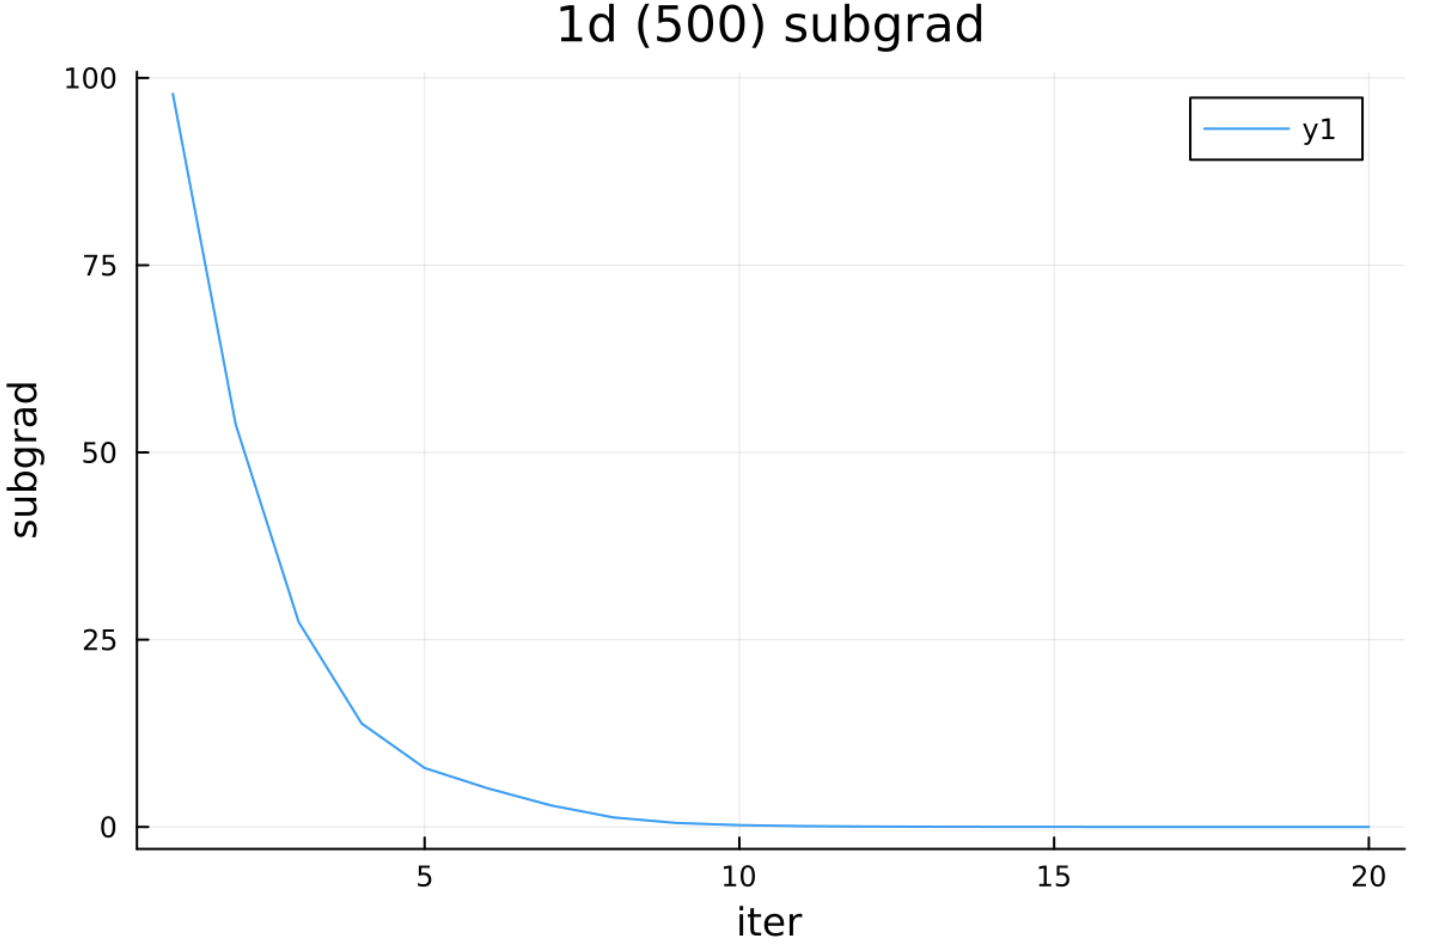
\includegraphics[width=0.3\textwidth]{1dsubgrad.png} 
			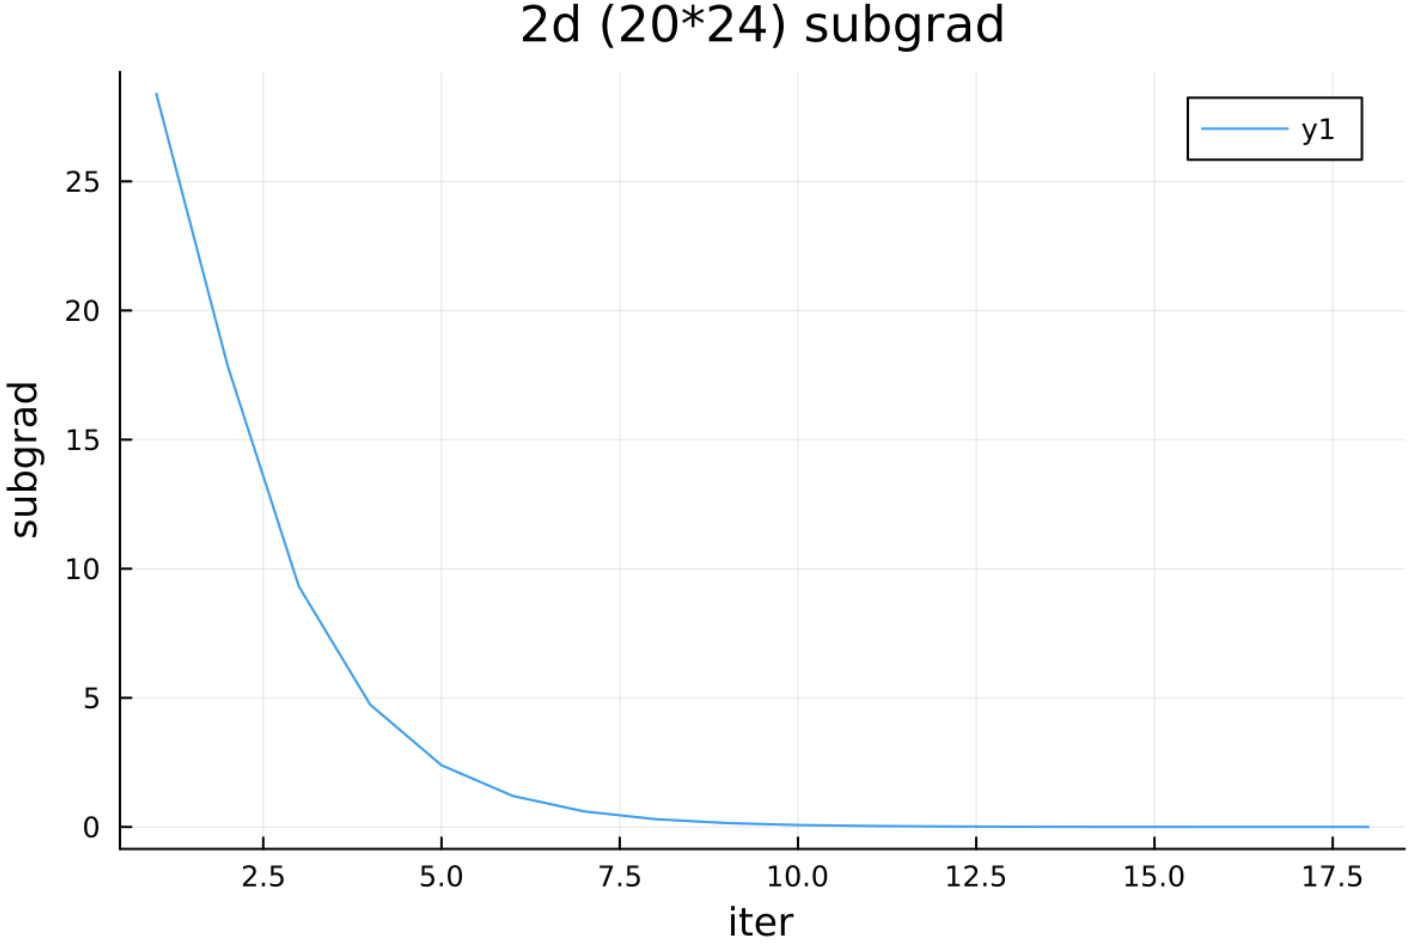
\includegraphics[width=0.3\textwidth]{2dsubgrad.png}
          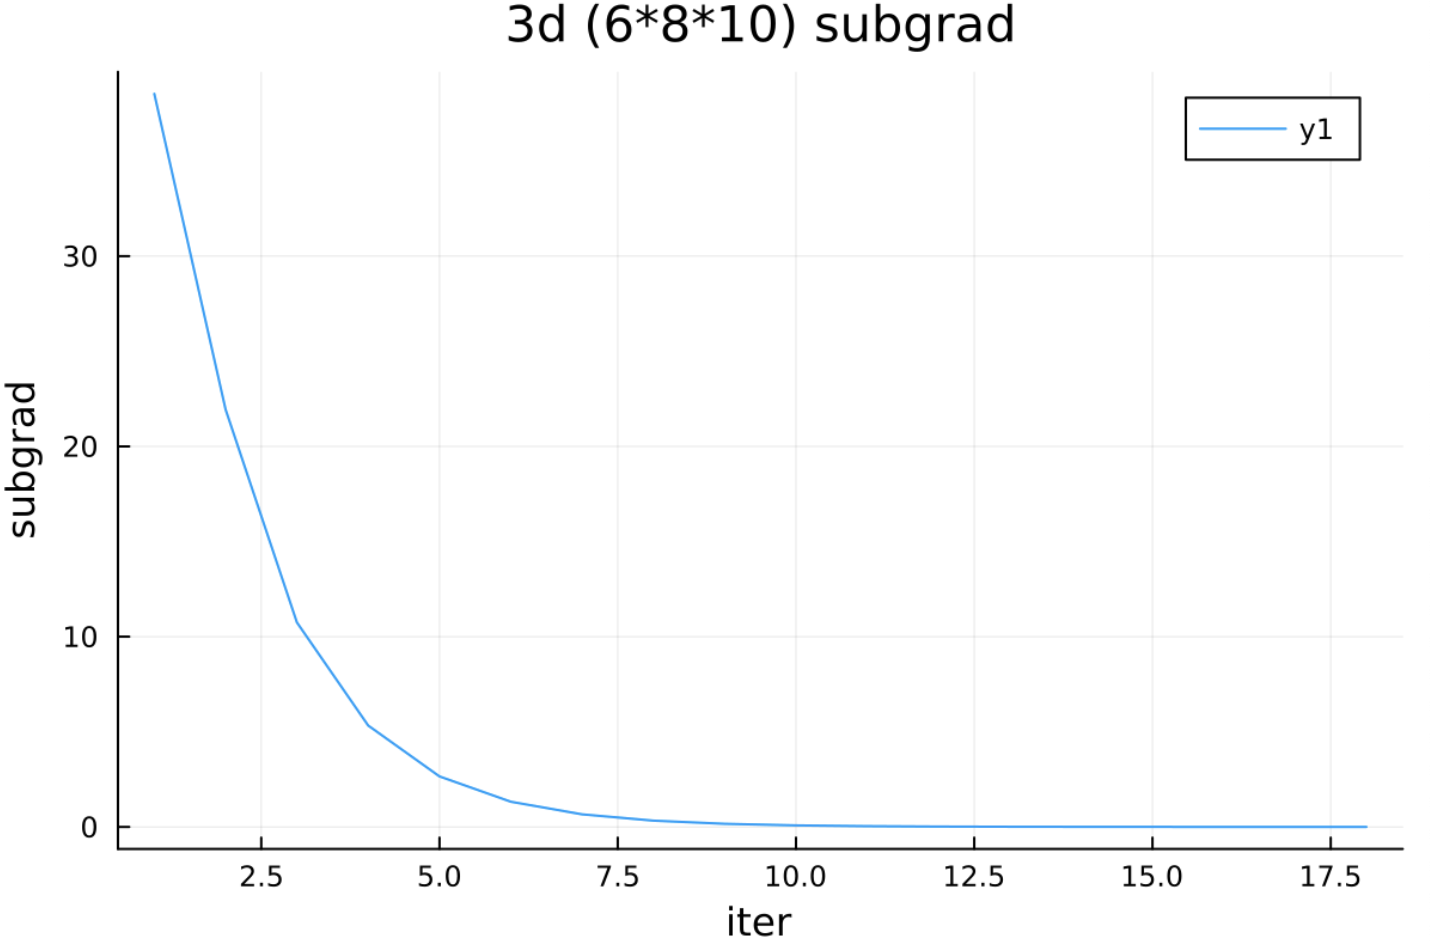
\includegraphics[width=0.3\textwidth]{3dsubgrad.png}
		\end{minipage}
	}
    	\subfigure{
    		\begin{minipage}[b]{1\textwidth}
   		 	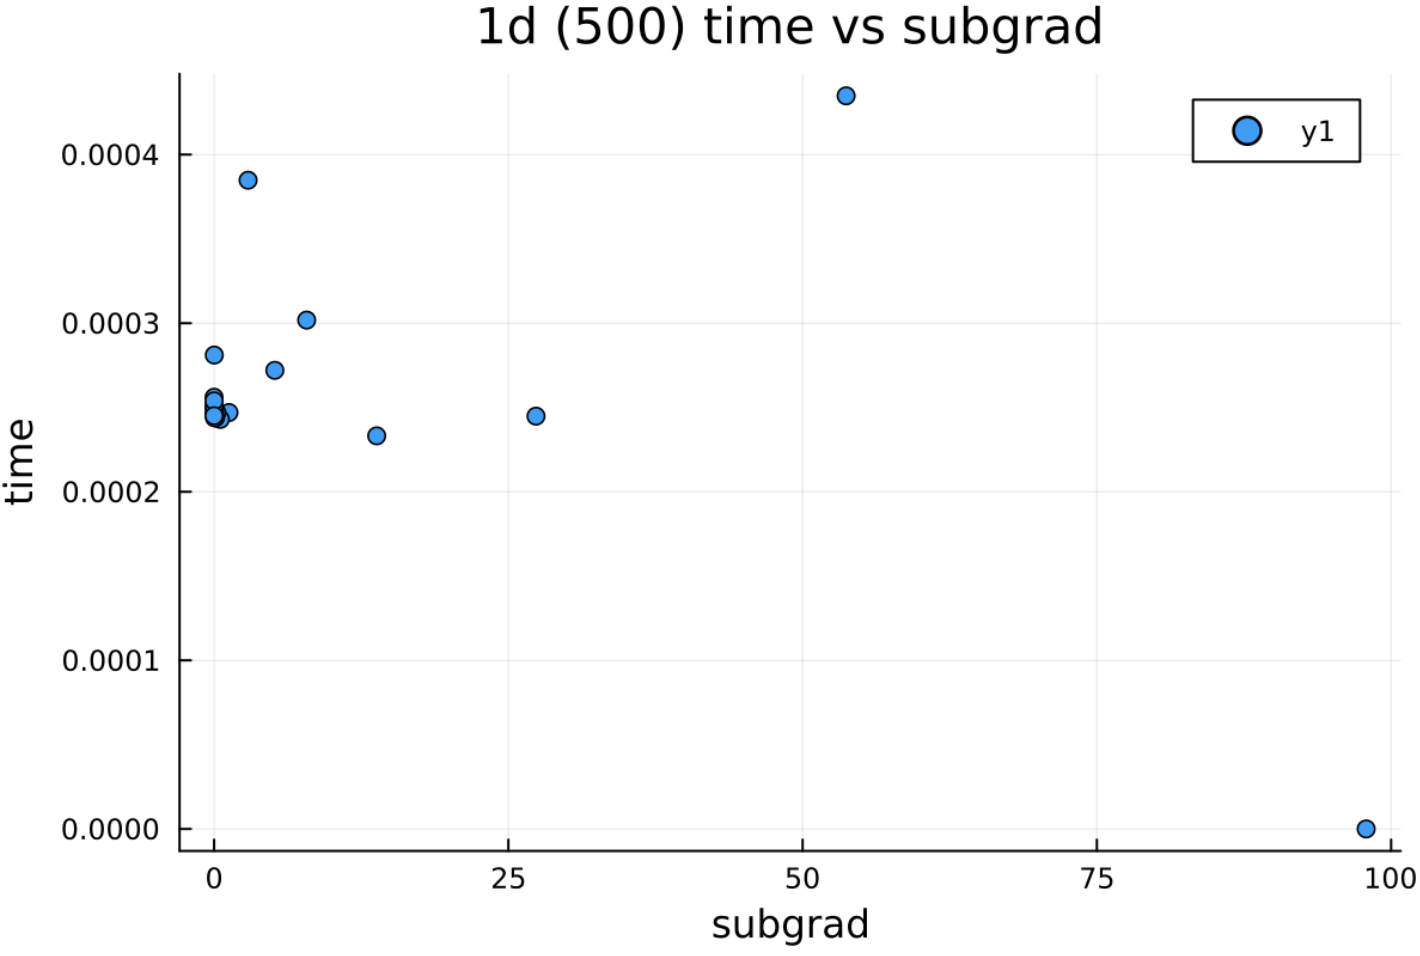
\includegraphics[width=0.3\textwidth]{1dtimevssubgrad.png}
		 	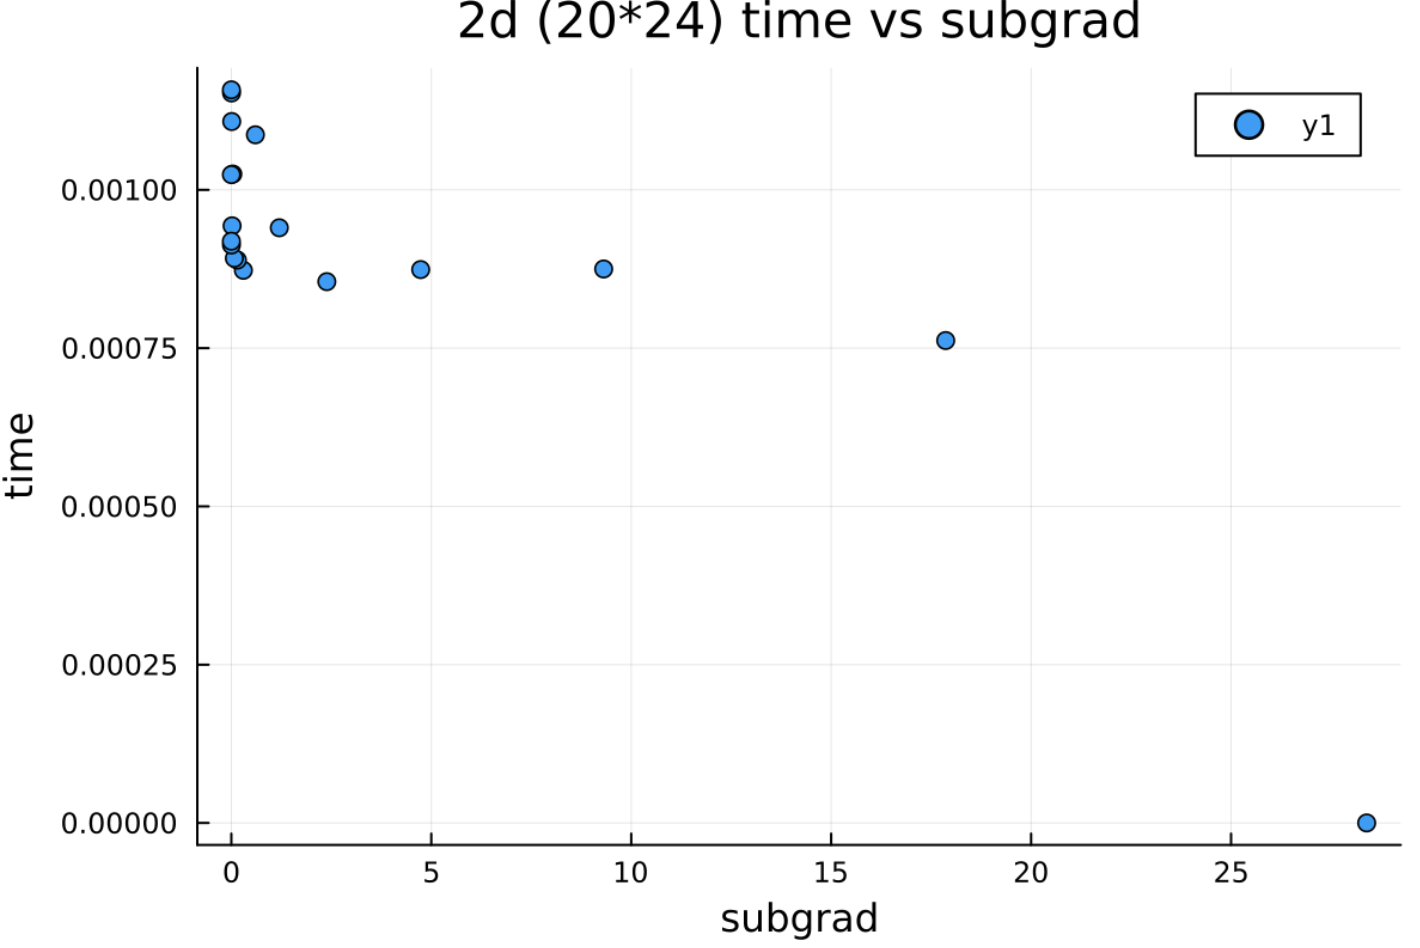
\includegraphics[width=0.3\textwidth]{2dtimevssubgrad.png}
            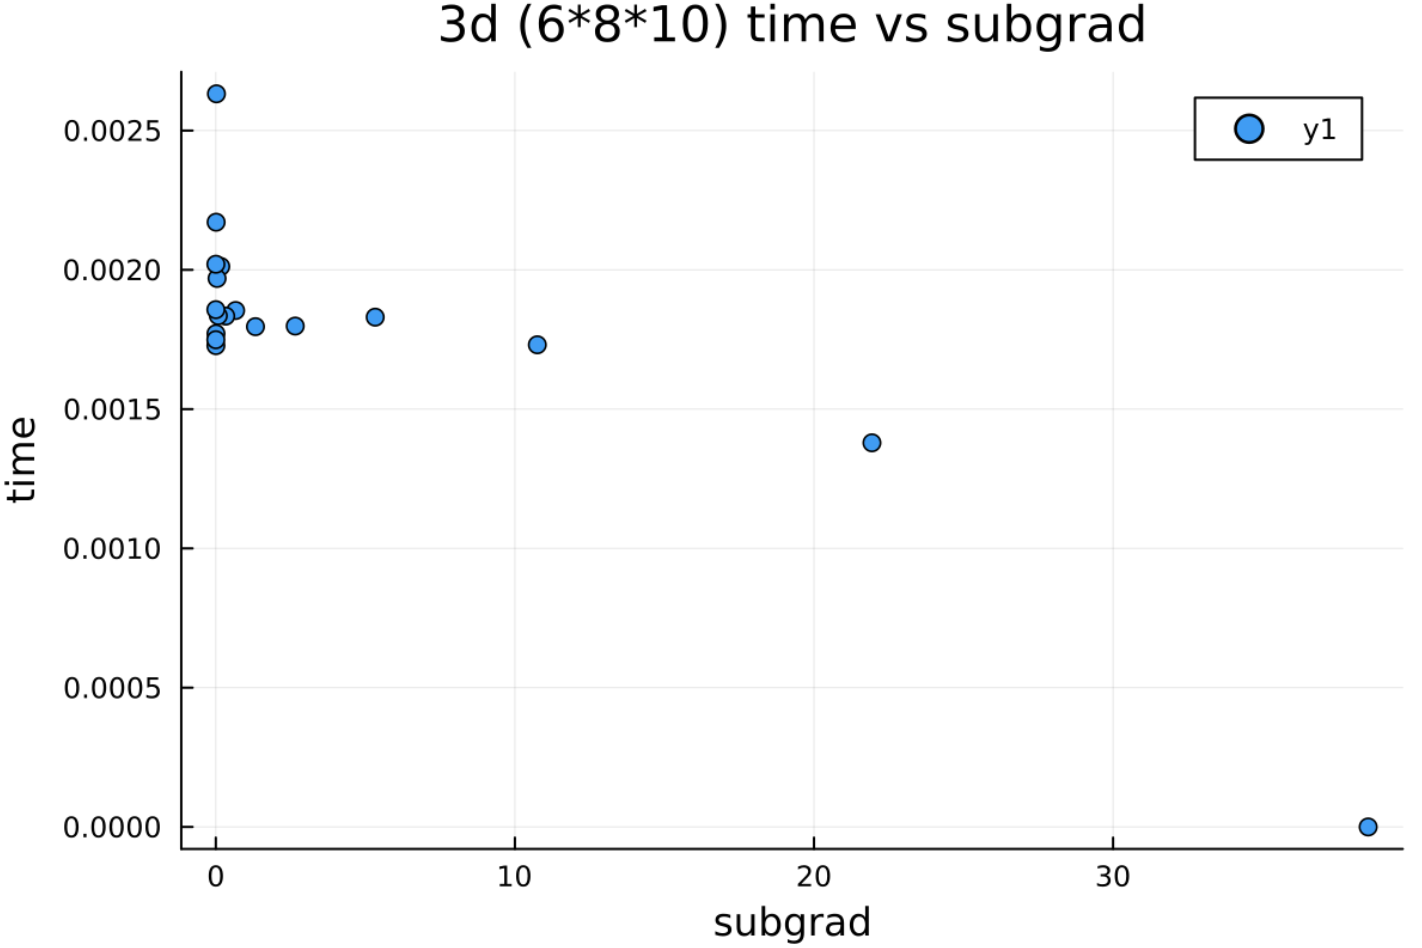
\includegraphics[width=0.3\textwidth]{3dtimevssubgrad.png}
    		\end{minipage}
		}
\end{figure}

\section{IPOPT}
We start with the problem
\begin{equation}
    \min_{\beta} \frac{1}{2}\|z-M_{\perp}\beta\|^2 \text{ s.t }\|\beta\|_1\leq d,
\end{equation}
the Lagrangian of which is
\begin{equation}
    L(\beta, \lambda) = \frac{1}{2}\|z-M_{\perp}\beta\|^2 + \lambda(\|\beta\|_1-d).
\end{equation}
Therefore,
\begin{equation}
   \beta^\star = \arg\min_{\beta} L(\beta, \lambda^\star) \quad\Rightarrow \quad\partial_{\beta} L(\beta, \lambda^\star) = 0. 
\end{equation}
To make the constraint differentiable, we rewrite the problem as
\begin{equation}
    \begin{aligned}
        \min_{\beta} &\frac{1}{2}\|z-M_{\perp}\beta\|^2\\
        \text{s.t. }&l_i = -\beta_i-c_i\leq 0\\
        &u_i = \beta_i-c_i\leq 0\\
        &h_i = -c_i\leq 0\\
        &g = \sum_{i}c_i-d\leq 0
    \end{aligned}
\end{equation}
Now the Lagrangian becomes
\begin{equation}
    L(\beta,c; \xi,\eta,\nu,\lambda)= 
     \frac{1}{2}\|z-M_{\perp}\beta\|^2
     +\sum_{i}\xi_i(-\beta_i-c_i)
     +\sum_{i}\eta_i(\beta_i-c_i)
     +\sum_{i}\nu_i(-c_i) + \lambda(\sum_{i}c_i-d).
\end{equation}
$\beta^\star, c^\star$ are the minimizer given $\xi^\star, \eta^\star, \nu^\star, \lambda^\star$.

\section{Primal-Dual IPOPT}
If we consider the problem
\begin{equation}
    \min_x f_0(x) \text{ s.t. } f_i(x)\leq 0, i=1,\dots,m.
\end{equation}
The primal-dual IPOPT algorithm is given as
\begin{figure}[H]
	\centering	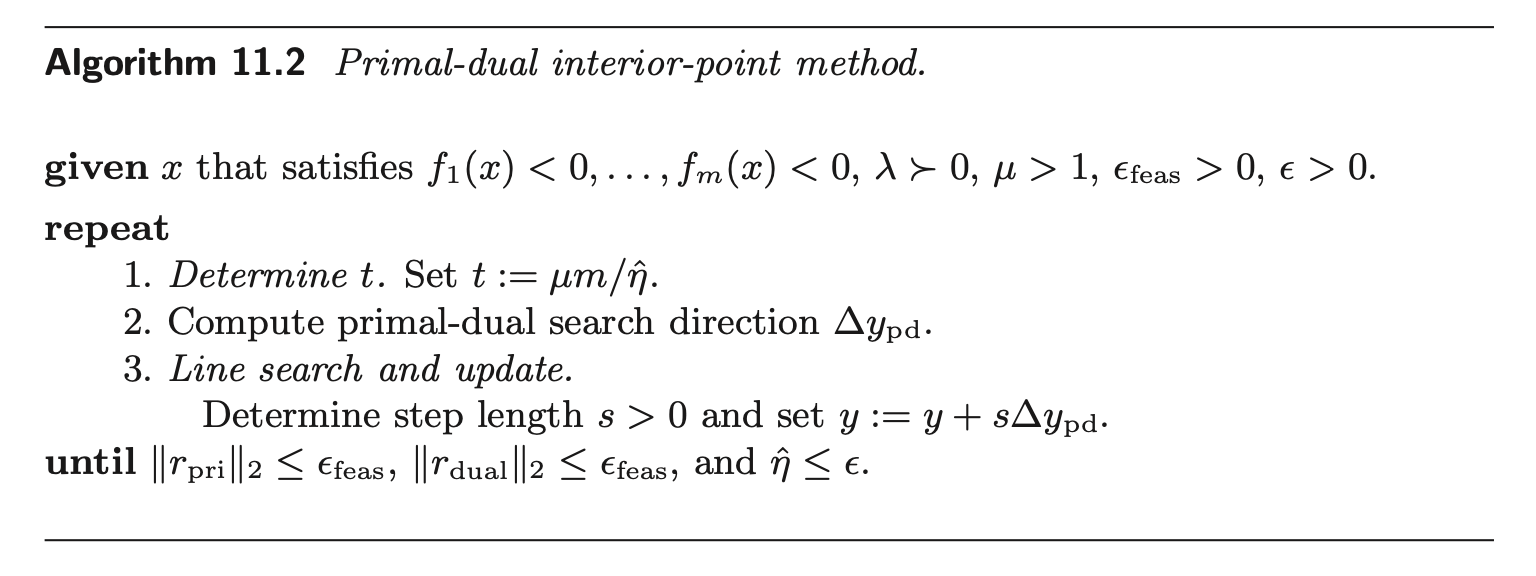
\includegraphics[width=0.7\textwidth]{PDIPOPT.png} 
\end{figure}

Adapt it to our problem, the computation details is as follows: Denote
\begin{equation}
    f(x) = (f_1(x),\dots,f_m(x))^T\text{ and }Df(x)^T = (\nabla f_1(x),\dots,\nabla f_m(x)).
\end{equation}
Define
\begin{equation}
    r_t(x,\lambda) = \begin{pmatrix}
    \nabla f_0(x)+Df(x)^T\lambda\\
    -diag(\lambda)f(x)-\frac{1}{t}\boldsymbol{1}
    \end{pmatrix}=:\begin{pmatrix}
        r_{\text{dual}}\\
        r_{\text{cent}}
    \end{pmatrix}.
\end{equation}
The system we need to solve is
\begin{equation}
    r_t(y+\Delta y) \approx r_t(y)+D r_t(y) \Delta y=0 \Rightarrow \Delta y=-D r_t(y)^{-1} r_t(y).
\end{equation}
Plug in the definition of $r_t$, we have
\begin{equation}
    \left(\begin{array}{cc}
\nabla^2 f_0(x)+\sum_{i=1}^m \lambda_i \nabla^2 f_i(x) & D f(x)^{T} \\
-\operatorname{diag}(\lambda) D f(x) & -\operatorname{diag}(f(x))
\end{array}\right)\left(\begin{array}{c}
\Delta x \\
\Delta \lambda
\end{array}\right)=-\left(\begin{array}{c}
r_{\text {dual }} \\
r_{\text {cent }}
\end{array}\right)
\end{equation}
From the second line, we can represent $\Delta \lambda$ with $\Delta x$:
\begin{equation}
    \Delta \lambda = -\operatorname{diag}(f(x))^{-1} \operatorname{diag}(x) D f(x) \Delta x+\operatorname{diag}(f(x))^{-1} r_{\text {cent }}.
\end{equation}
Plug it back into the first line, we have
\begin{equation}
    \left(\nabla^2 f_0(x)+\sum_{i=1}^m \lambda_i \nabla^2 f_i(x)+\sum_{i=1}^m \frac{\lambda_i}{-f_i(x)} \nabla f_i(x) \nabla f_i(x)^{\top}\right) \Delta x=-\left(\nabla f_0(x)+\frac{1}{t} \sum_{i=1}^m \frac{1}{-f_i(x)} \nabla f_i(x)\right).
\end{equation}
Now we consider our problem, we know the matrix
\begin{equation}
    \begin{aligned}
        &\nabla^2 f_0(x)+\sum_{i=1}^m \lambda_i \nabla^2 f_i(x)+\sum_{i=1}^m \frac{\lambda_i}{-f_i(x)} \nabla f_i(x) \nabla f_i(x)^{\top}\\
        &=\left(\begin{array}{ll}
M_{\perp}^{\top} M_{\perp}+\operatorname{diag}\left(-\frac{\lambda}{l}-\frac{\xi}{u}\right) & \operatorname{diag}\left(-\frac{\lambda}{l}+\frac{\xi}{u}\right) \\
\operatorname{diag}\left(-\frac{\lambda}{l}+\frac{\xi}{u}\right) & \operatorname{diag}\left(-\frac{\lambda}{l}-\frac{\xi}{u}-\frac{\eta}{h}\right)-\frac{\nu}{g} 11^{\top}
\end{array}\right),
    \end{aligned}
\end{equation}
where $\lambda$, $\xi$, $\eta$, and $\nu$
 are the dual variables corresponding to $l, u, h, g$, respectively. The matrix used for preconditioner in CG is
 \begin{equation}
     \left(\begin{array}{ll}
I+\operatorname{diag}\left(-\frac{\lambda}{l}-\frac{\xi}{u}\right) & \operatorname{diag}\left(-\frac{\lambda}{l}+\frac{\xi}{u}\right) \\
\operatorname{diag}\left(-\frac{\lambda}{l}+\frac{\xi}{u}\right) & \operatorname{diag}\left(-\frac{\lambda}{l}-\frac{\xi}{u}-\frac{\eta}{h}\right)
\end{array}\right)
 \end{equation}
 Also, we have
 \begin{equation}
     -\left(\nabla f_0(x)+\frac{1}{t} \sum_{i=1}^m \frac{1}{-f_i(x)} \nabla f_i(x)\right)=\left(\begin{array}{c}
-M_{\perp}^{\top} M_{\perp} \beta+M_{\perp}^{\top} z+\frac{1}{t}\left(-\frac{1}{l}+\frac{1}{n}\right) \\
\frac{1}{t}\left(-\frac{1}{l}-\frac{1}{u}-\frac{1}{h}+\frac{1}{g} 1\right)
\end{array}\right).
 \end{equation}
 Thus, the search direction for dual variable is
 \begin{equation}
     -\left(\begin{array}{c}
\frac{\lambda}{l(x)} \\
\frac{\xi}{\mu(x)} \\
\frac{\eta}{h(x)} \\
\frac{v}{g(x)}
\end{array}\right) \odot\left(\begin{array}{c}
-\Delta \beta-\Delta c \\
\Delta \beta-\Delta c \\
-\Delta c \\
\boldsymbol{1}^{\top} \Delta c
\end{array}\right)-\left(\begin{array}{c}
\lambda \\
\xi \\
y \\
\nu
\end{array}\right)-\frac{1}{t}\left(\begin{array}{c}
\frac{1}{l} \\
\frac{1}{h} \\
\frac{1}{h} \\
\frac{1}{g}
\end{array}\right)
 \end{equation}
%References
%\printbibliography
%\appendix



\end{document}
